% Options for packages loaded elsewhere
\PassOptionsToPackage{unicode}{hyperref}
\PassOptionsToPackage{hyphens}{url}
%
\documentclass[
]{article}
\usepackage{amsmath,amssymb}
\usepackage{lmodern}
\usepackage{iftex}
\ifPDFTeX
  \usepackage[T1]{fontenc}
  \usepackage[utf8]{inputenc}
  \usepackage{textcomp} % provide euro and other symbols
\else % if luatex or xetex
  \usepackage{unicode-math}
  \defaultfontfeatures{Scale=MatchLowercase}
  \defaultfontfeatures[\rmfamily]{Ligatures=TeX,Scale=1}
\fi
% Use upquote if available, for straight quotes in verbatim environments
\IfFileExists{upquote.sty}{\usepackage{upquote}}{}
\IfFileExists{microtype.sty}{% use microtype if available
  \usepackage[]{microtype}
  \UseMicrotypeSet[protrusion]{basicmath} % disable protrusion for tt fonts
}{}
\makeatletter
\@ifundefined{KOMAClassName}{% if non-KOMA class
  \IfFileExists{parskip.sty}{%
    \usepackage{parskip}
  }{% else
    \setlength{\parindent}{0pt}
    \setlength{\parskip}{6pt plus 2pt minus 1pt}}
}{% if KOMA class
  \KOMAoptions{parskip=half}}
\makeatother
\usepackage{xcolor}
\IfFileExists{xurl.sty}{\usepackage{xurl}}{} % add URL line breaks if available
\IfFileExists{bookmark.sty}{\usepackage{bookmark}}{\usepackage{hyperref}}
\hypersetup{
  pdftitle={ATLANTIC CAMTRAPS - GRÁFICOS},
  pdfauthor={Fernando Lima},
  hidelinks,
  pdfcreator={LaTeX via pandoc}}
\urlstyle{same} % disable monospaced font for URLs
\usepackage[margin=1in]{geometry}
\usepackage{color}
\usepackage{fancyvrb}
\newcommand{\VerbBar}{|}
\newcommand{\VERB}{\Verb[commandchars=\\\{\}]}
\DefineVerbatimEnvironment{Highlighting}{Verbatim}{commandchars=\\\{\}}
% Add ',fontsize=\small' for more characters per line
\usepackage{framed}
\definecolor{shadecolor}{RGB}{248,248,248}
\newenvironment{Shaded}{\begin{snugshade}}{\end{snugshade}}
\newcommand{\AlertTok}[1]{\textcolor[rgb]{0.94,0.16,0.16}{#1}}
\newcommand{\AnnotationTok}[1]{\textcolor[rgb]{0.56,0.35,0.01}{\textbf{\textit{#1}}}}
\newcommand{\AttributeTok}[1]{\textcolor[rgb]{0.77,0.63,0.00}{#1}}
\newcommand{\BaseNTok}[1]{\textcolor[rgb]{0.00,0.00,0.81}{#1}}
\newcommand{\BuiltInTok}[1]{#1}
\newcommand{\CharTok}[1]{\textcolor[rgb]{0.31,0.60,0.02}{#1}}
\newcommand{\CommentTok}[1]{\textcolor[rgb]{0.56,0.35,0.01}{\textit{#1}}}
\newcommand{\CommentVarTok}[1]{\textcolor[rgb]{0.56,0.35,0.01}{\textbf{\textit{#1}}}}
\newcommand{\ConstantTok}[1]{\textcolor[rgb]{0.00,0.00,0.00}{#1}}
\newcommand{\ControlFlowTok}[1]{\textcolor[rgb]{0.13,0.29,0.53}{\textbf{#1}}}
\newcommand{\DataTypeTok}[1]{\textcolor[rgb]{0.13,0.29,0.53}{#1}}
\newcommand{\DecValTok}[1]{\textcolor[rgb]{0.00,0.00,0.81}{#1}}
\newcommand{\DocumentationTok}[1]{\textcolor[rgb]{0.56,0.35,0.01}{\textbf{\textit{#1}}}}
\newcommand{\ErrorTok}[1]{\textcolor[rgb]{0.64,0.00,0.00}{\textbf{#1}}}
\newcommand{\ExtensionTok}[1]{#1}
\newcommand{\FloatTok}[1]{\textcolor[rgb]{0.00,0.00,0.81}{#1}}
\newcommand{\FunctionTok}[1]{\textcolor[rgb]{0.00,0.00,0.00}{#1}}
\newcommand{\ImportTok}[1]{#1}
\newcommand{\InformationTok}[1]{\textcolor[rgb]{0.56,0.35,0.01}{\textbf{\textit{#1}}}}
\newcommand{\KeywordTok}[1]{\textcolor[rgb]{0.13,0.29,0.53}{\textbf{#1}}}
\newcommand{\NormalTok}[1]{#1}
\newcommand{\OperatorTok}[1]{\textcolor[rgb]{0.81,0.36,0.00}{\textbf{#1}}}
\newcommand{\OtherTok}[1]{\textcolor[rgb]{0.56,0.35,0.01}{#1}}
\newcommand{\PreprocessorTok}[1]{\textcolor[rgb]{0.56,0.35,0.01}{\textit{#1}}}
\newcommand{\RegionMarkerTok}[1]{#1}
\newcommand{\SpecialCharTok}[1]{\textcolor[rgb]{0.00,0.00,0.00}{#1}}
\newcommand{\SpecialStringTok}[1]{\textcolor[rgb]{0.31,0.60,0.02}{#1}}
\newcommand{\StringTok}[1]{\textcolor[rgb]{0.31,0.60,0.02}{#1}}
\newcommand{\VariableTok}[1]{\textcolor[rgb]{0.00,0.00,0.00}{#1}}
\newcommand{\VerbatimStringTok}[1]{\textcolor[rgb]{0.31,0.60,0.02}{#1}}
\newcommand{\WarningTok}[1]{\textcolor[rgb]{0.56,0.35,0.01}{\textbf{\textit{#1}}}}
\usepackage{graphicx}
\makeatletter
\def\maxwidth{\ifdim\Gin@nat@width>\linewidth\linewidth\else\Gin@nat@width\fi}
\def\maxheight{\ifdim\Gin@nat@height>\textheight\textheight\else\Gin@nat@height\fi}
\makeatother
% Scale images if necessary, so that they will not overflow the page
% margins by default, and it is still possible to overwrite the defaults
% using explicit options in \includegraphics[width, height, ...]{}
\setkeys{Gin}{width=\maxwidth,height=\maxheight,keepaspectratio}
% Set default figure placement to htbp
\makeatletter
\def\fps@figure{htbp}
\makeatother
\setlength{\emergencystretch}{3em} % prevent overfull lines
\providecommand{\tightlist}{%
  \setlength{\itemsep}{0pt}\setlength{\parskip}{0pt}}
\setcounter{secnumdepth}{-\maxdimen} % remove section numbering
\ifLuaTeX
  \usepackage{selnolig}  % disable illegal ligatures
\fi

\title{ATLANTIC CAMTRAPS - GRÁFICOS}
\author{Fernando Lima}
\date{9 de novembro de 2017}

\begin{document}
\maketitle

\begin{Shaded}
\begin{Highlighting}[]
\FunctionTok{library}\NormalTok{(here)}
\end{Highlighting}
\end{Shaded}

\begin{verbatim}
## here() starts at D:/git/atlantic-series/ATLANTIC_CAMTRAP
\end{verbatim}

\begin{Shaded}
\begin{Highlighting}[]
\FunctionTok{library}\NormalTok{(ggplot2)}
\FunctionTok{library}\NormalTok{(forcats)}
\FunctionTok{library}\NormalTok{(RColorBrewer)}
\end{Highlighting}
\end{Shaded}

\hypertarget{descriuxe7uxe3o}{%
\subsection{DESCRIÇÃO}\label{descriuxe7uxe3o}}

Gráficos para o datapaper Atlantic-Camtraps. Adaptado e organizado a
partir da primeira versão criada por Renata Muylaert.

\hypertarget{grupo-de-trabalho}{%
\subsubsection{GRUPO DE TRABALHO}\label{grupo-de-trabalho}}

\textbf{pH} Fernando Lima, D.Sc.\\
\textbf{RM} Renata Muylaert, D.Sc.\\
\textbf{MR} Milton Ribeiro, D.Sc.

\hypertarget{notas-readme}{%
\subsubsection{NOTAS (README)}\label{notas-readme}}

ADICAO DE COMENTARIOS: Corpo do Texto: insira suas iniciais entre
\texttt{**} e depois os comentarios: e.g.~\texttt{**pH**} blablabla
Código:

\hypertarget{data-prep}{%
\subsubsection{Data prep}\label{data-prep}}

\#\#\#\#Select species and effort data

\begin{Shaded}
\begin{Highlighting}[]
\NormalTok{data }\OtherTok{\textless{}{-}} \FunctionTok{read.csv}\NormalTok{(}\FunctionTok{here}\NormalTok{(}\StringTok{"data"}\NormalTok{, }\StringTok{"splist\_filtered\_2017\_04d24.csv"}\NormalTok{), }\AttributeTok{sep =} \StringTok{","}\NormalTok{)}
\NormalTok{ef }\OtherTok{\textless{}{-}} \FunctionTok{read.csv}\NormalTok{(}\FunctionTok{here}\NormalTok{(}\StringTok{"data"}\NormalTok{, }\StringTok{"effort.txt"}\NormalTok{), }\AttributeTok{sep=}\StringTok{"}\SpecialCharTok{\textbackslash{}t}\StringTok{"}\NormalTok{)}
\end{Highlighting}
\end{Shaded}

\#\#\#\#Ordenando data por ordem e por FO:

\begin{Shaded}
\begin{Highlighting}[]
\NormalTok{data }\OtherTok{\textless{}{-}}\NormalTok{ data[}\FunctionTok{order}\NormalTok{(data}\SpecialCharTok{$}\NormalTok{fo),]}

\FunctionTok{str}\NormalTok{(data)}
\end{Highlighting}
\end{Shaded}

\begin{verbatim}
## 'data.frame':    47 obs. of  11 variables:
##  $ sp_id      : int  1032 1038 1022 1078 1079 1028 1035 1080 1081 1013 ...
##  $ class      : Factor w/ 1 level "Mammalia": 1 1 1 1 1 1 1 1 1 1 ...
##  $ order      : Factor w/ 8 levels "Artiodactyla",..: 3 3 2 8 8 2 3 8 8 2 ...
##  $ family     : Factor w/ 17 levels "Canidae","Caviidae",..: 5 5 11 8 8 14 5 8 8 1 ...
##  $ genus      : Factor w/ 36 levels "Cabassous","Canis",..: 1 27 7 4 6 26 10 31 31 30 ...
##  $ species    : Factor w/ 47 levels "albiventris",..: 43 23 10 36 31 15 34 20 45 44 ...
##  $ species.1  : Factor w/ 47 levels "Cabassous tatouay",..: 2 36 8 5 7 35 14 41 42 40 ...
##  $ iucn_status: Factor w/ 5 levels "DD","IN","LC",..: 3 5 3 5 3 3 3 3 3 4 ...
##  $ sp_code1   : Factor w/ 47 levels "Caba_tato","Caba_unic",..: 2 36 8 5 7 35 14 41 42 40 ...
##  $ sp_code    : Factor w/ 47 levels "Caba_tato","Caba_unic",..: 2 36 8 5 7 35 14 41 42 40 ...
##  $ fo         : num  0.00694 0.00694 0.01389 0.01389 0.01389 ...
\end{verbatim}

\begin{Shaded}
\begin{Highlighting}[]
\FunctionTok{unique}\NormalTok{(data}\SpecialCharTok{$}\NormalTok{sp\_id)}
\end{Highlighting}
\end{Shaded}

\begin{verbatim}
##  [1] 1032 1038 1022 1078 1079 1028 1035 1080 1081 1013 1012 1023 1011 1074 1026
## [16] 1019 1051 1014 1055 1008 1004 1037 1006 1025 1002 1031 1053 1003 1052 1021
## [31] 1017 1039 1068 1007 1020 1073 1040 1056 1015 1016 1072 1029 1009 1024 1010
## [46] 1027 1034
\end{verbatim}

\begin{Shaded}
\begin{Highlighting}[]
\FunctionTok{head}\NormalTok{(data)}
\end{Highlighting}
\end{Shaded}

\begin{verbatim}
##    sp_id    class     order         family      genus     species
## 28  1032 Mammalia Cingulata    Dasypodidae  Cabassous  unicinctus
## 32  1038 Mammalia Cingulata    Dasypodidae Priodontes     maximus
## 19  1022 Mammalia Carnivora     Mephitidae  Conepatus      chinga
## 44  1078 Mammalia  Rodentia Erethizontidae  Chaetomys subspinosus
## 45  1079 Mammalia  Rodentia Erethizontidae    Coendou prehensilis
## 25  1028 Mammalia Carnivora    Procyonidae      Potos      flavus
##                species.1 iucn_status  sp_code1   sp_code      fo
## 28  Cabassous unicinctus          LC Caba_unic Caba_unic 0.00694
## 32    Priodontes maximus          VU Prio_maxi Prio_maxi 0.00694
## 19      Conepatus chinga          LC Cone_chin Cone_chin 0.01389
## 44 Chaetomys subspinosus          VU Chae_subs Chae_subs 0.01389
## 45   Coendou prehensilis          LC Coen_preh Coen_preh 0.01389
## 25          Potos flavus          LC Poto_flav Potu_flav 0.02083
\end{verbatim}

\#\#\#FIGURE 01 - MAP

Generated in ArcGis by Fernando Lima

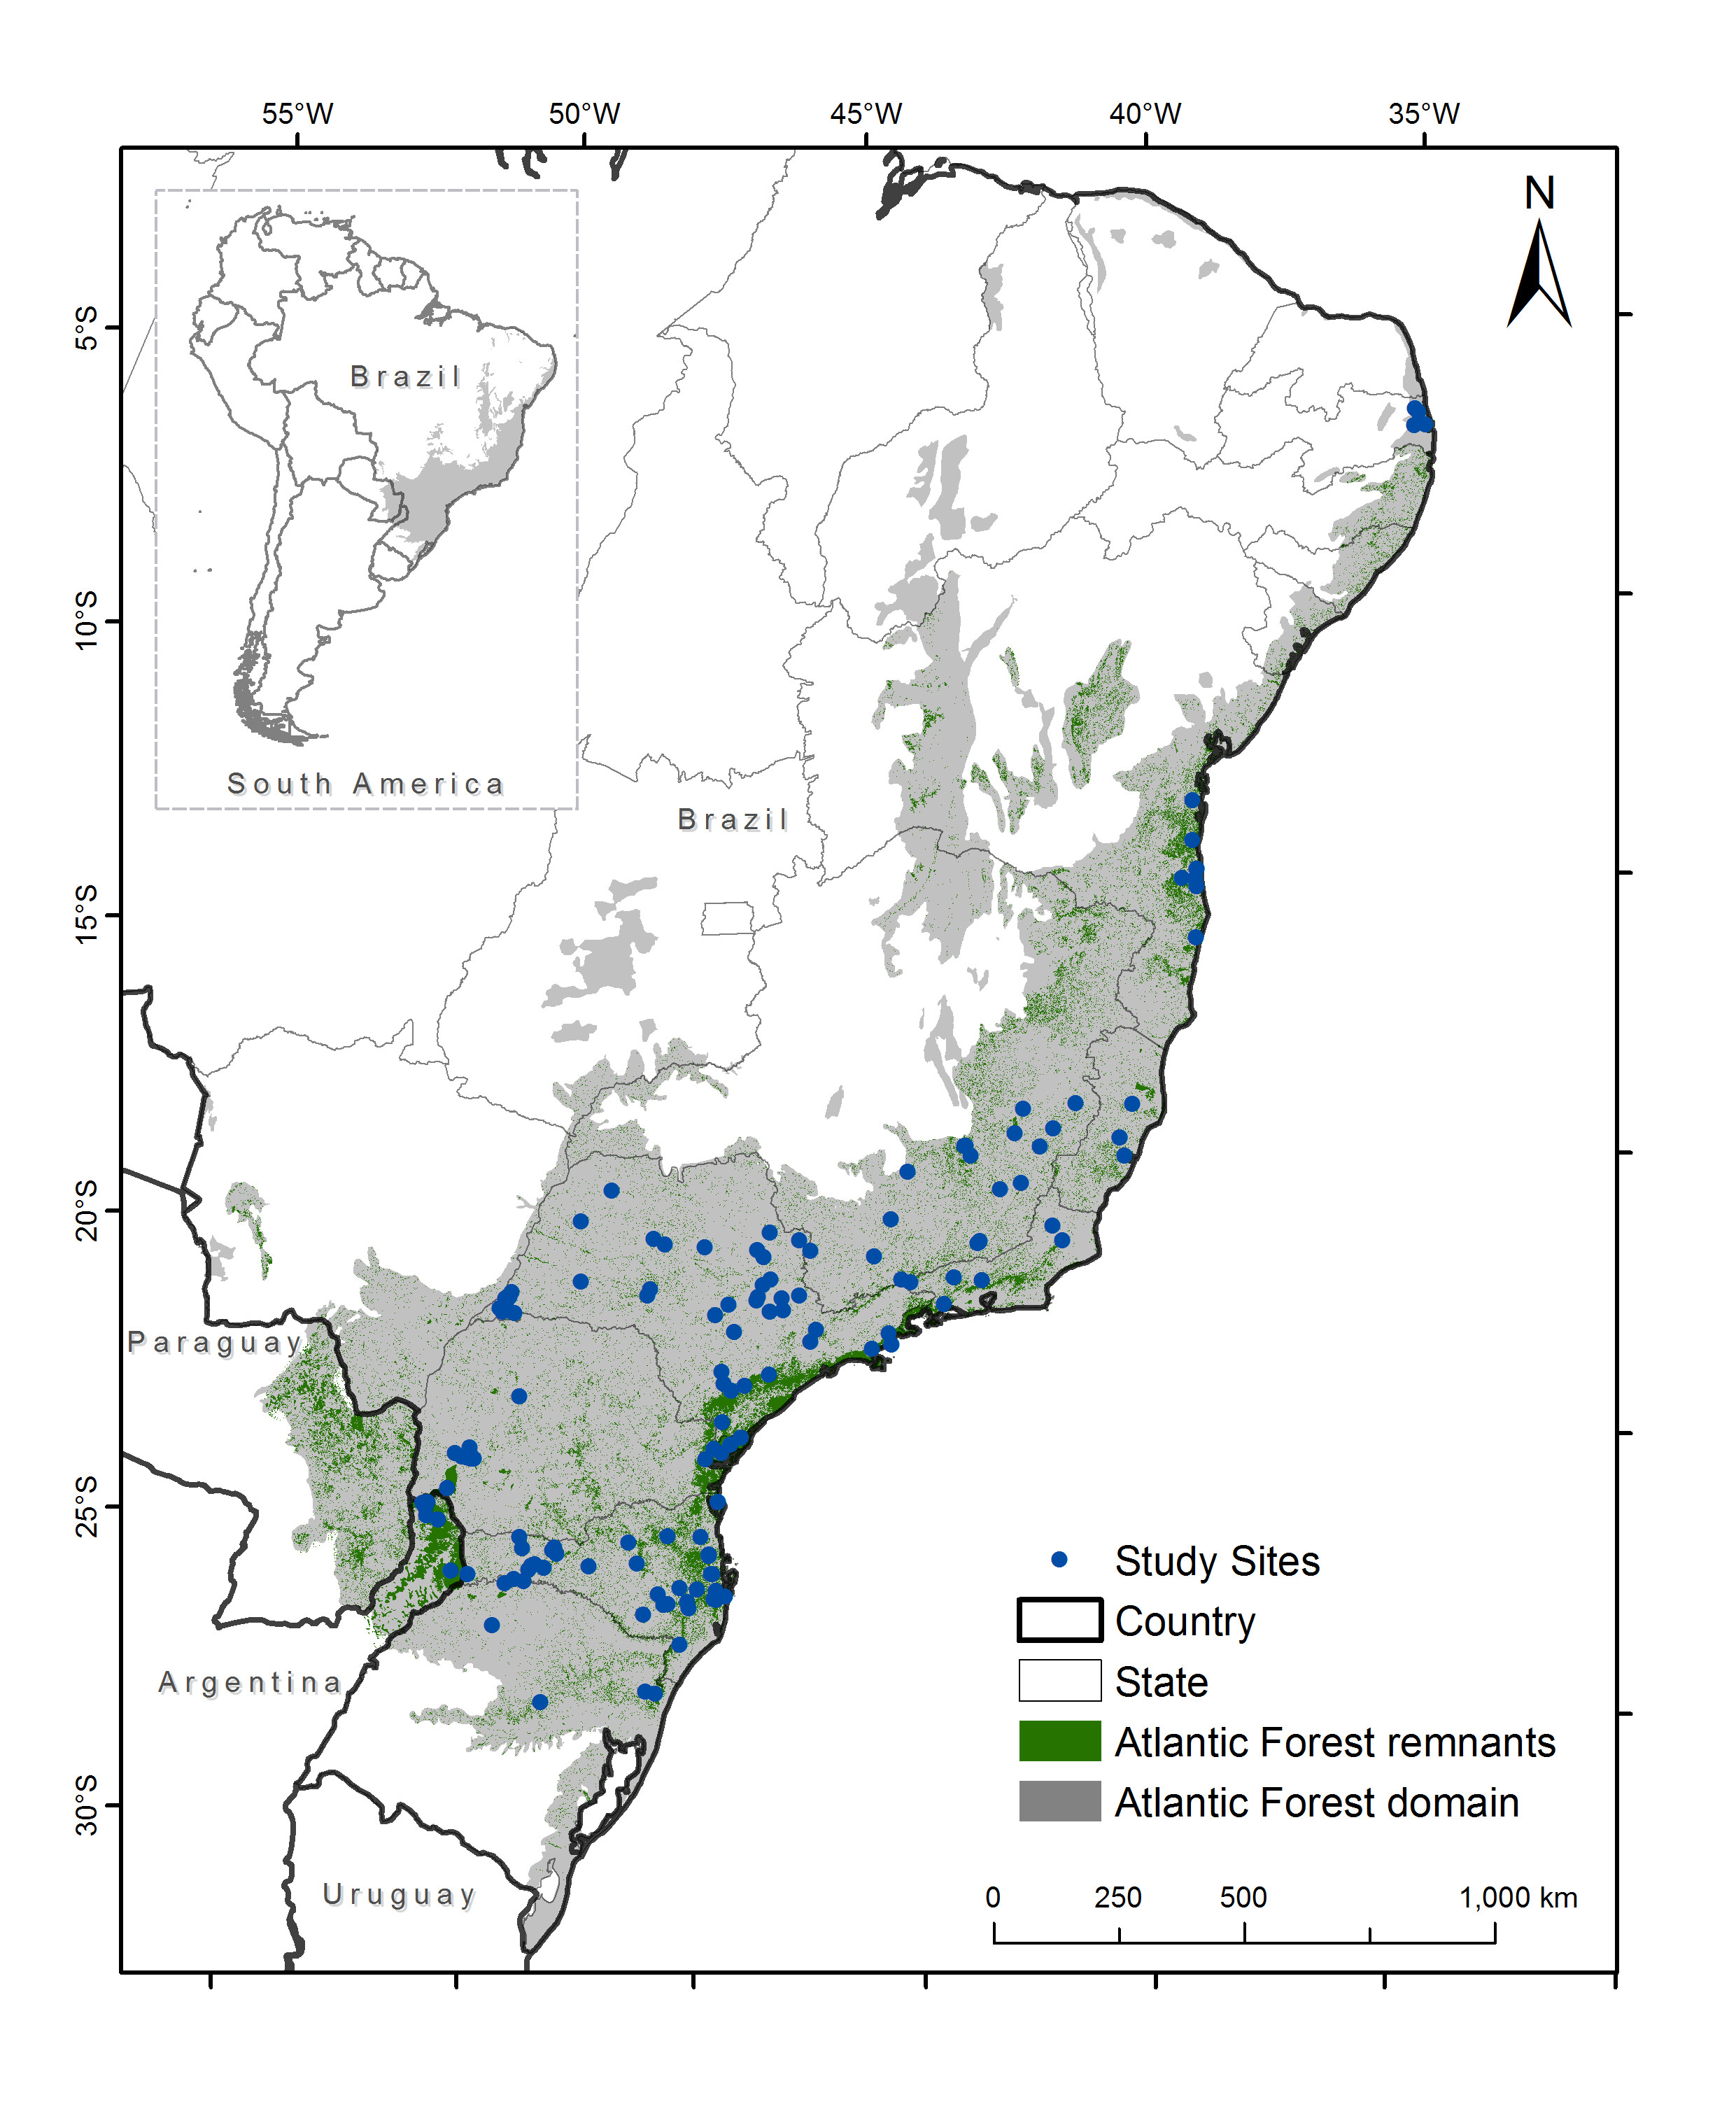
\includegraphics[width=700px]{D:/git/atlantic-series/ATLANTIC_CAMTRAP/figures/ATLANTIC_CAMTRAPS_FIG01}
\textbf{Fig. 1.} Distribution of the camera trap surveys of medium and
large terrestrial mammal communities within the Atlantic Forest extent.
Gray shows the Atlantic Forest extent with remaining forest patches in
green (sensu Ribeiro et al.~2009). Blue dots show the geographic
locations of studies.

\#\#\#FIGURA 02 - SUNBURST

Esta figura foi feita no Excel, utilizando a função \texttt{sunburst}

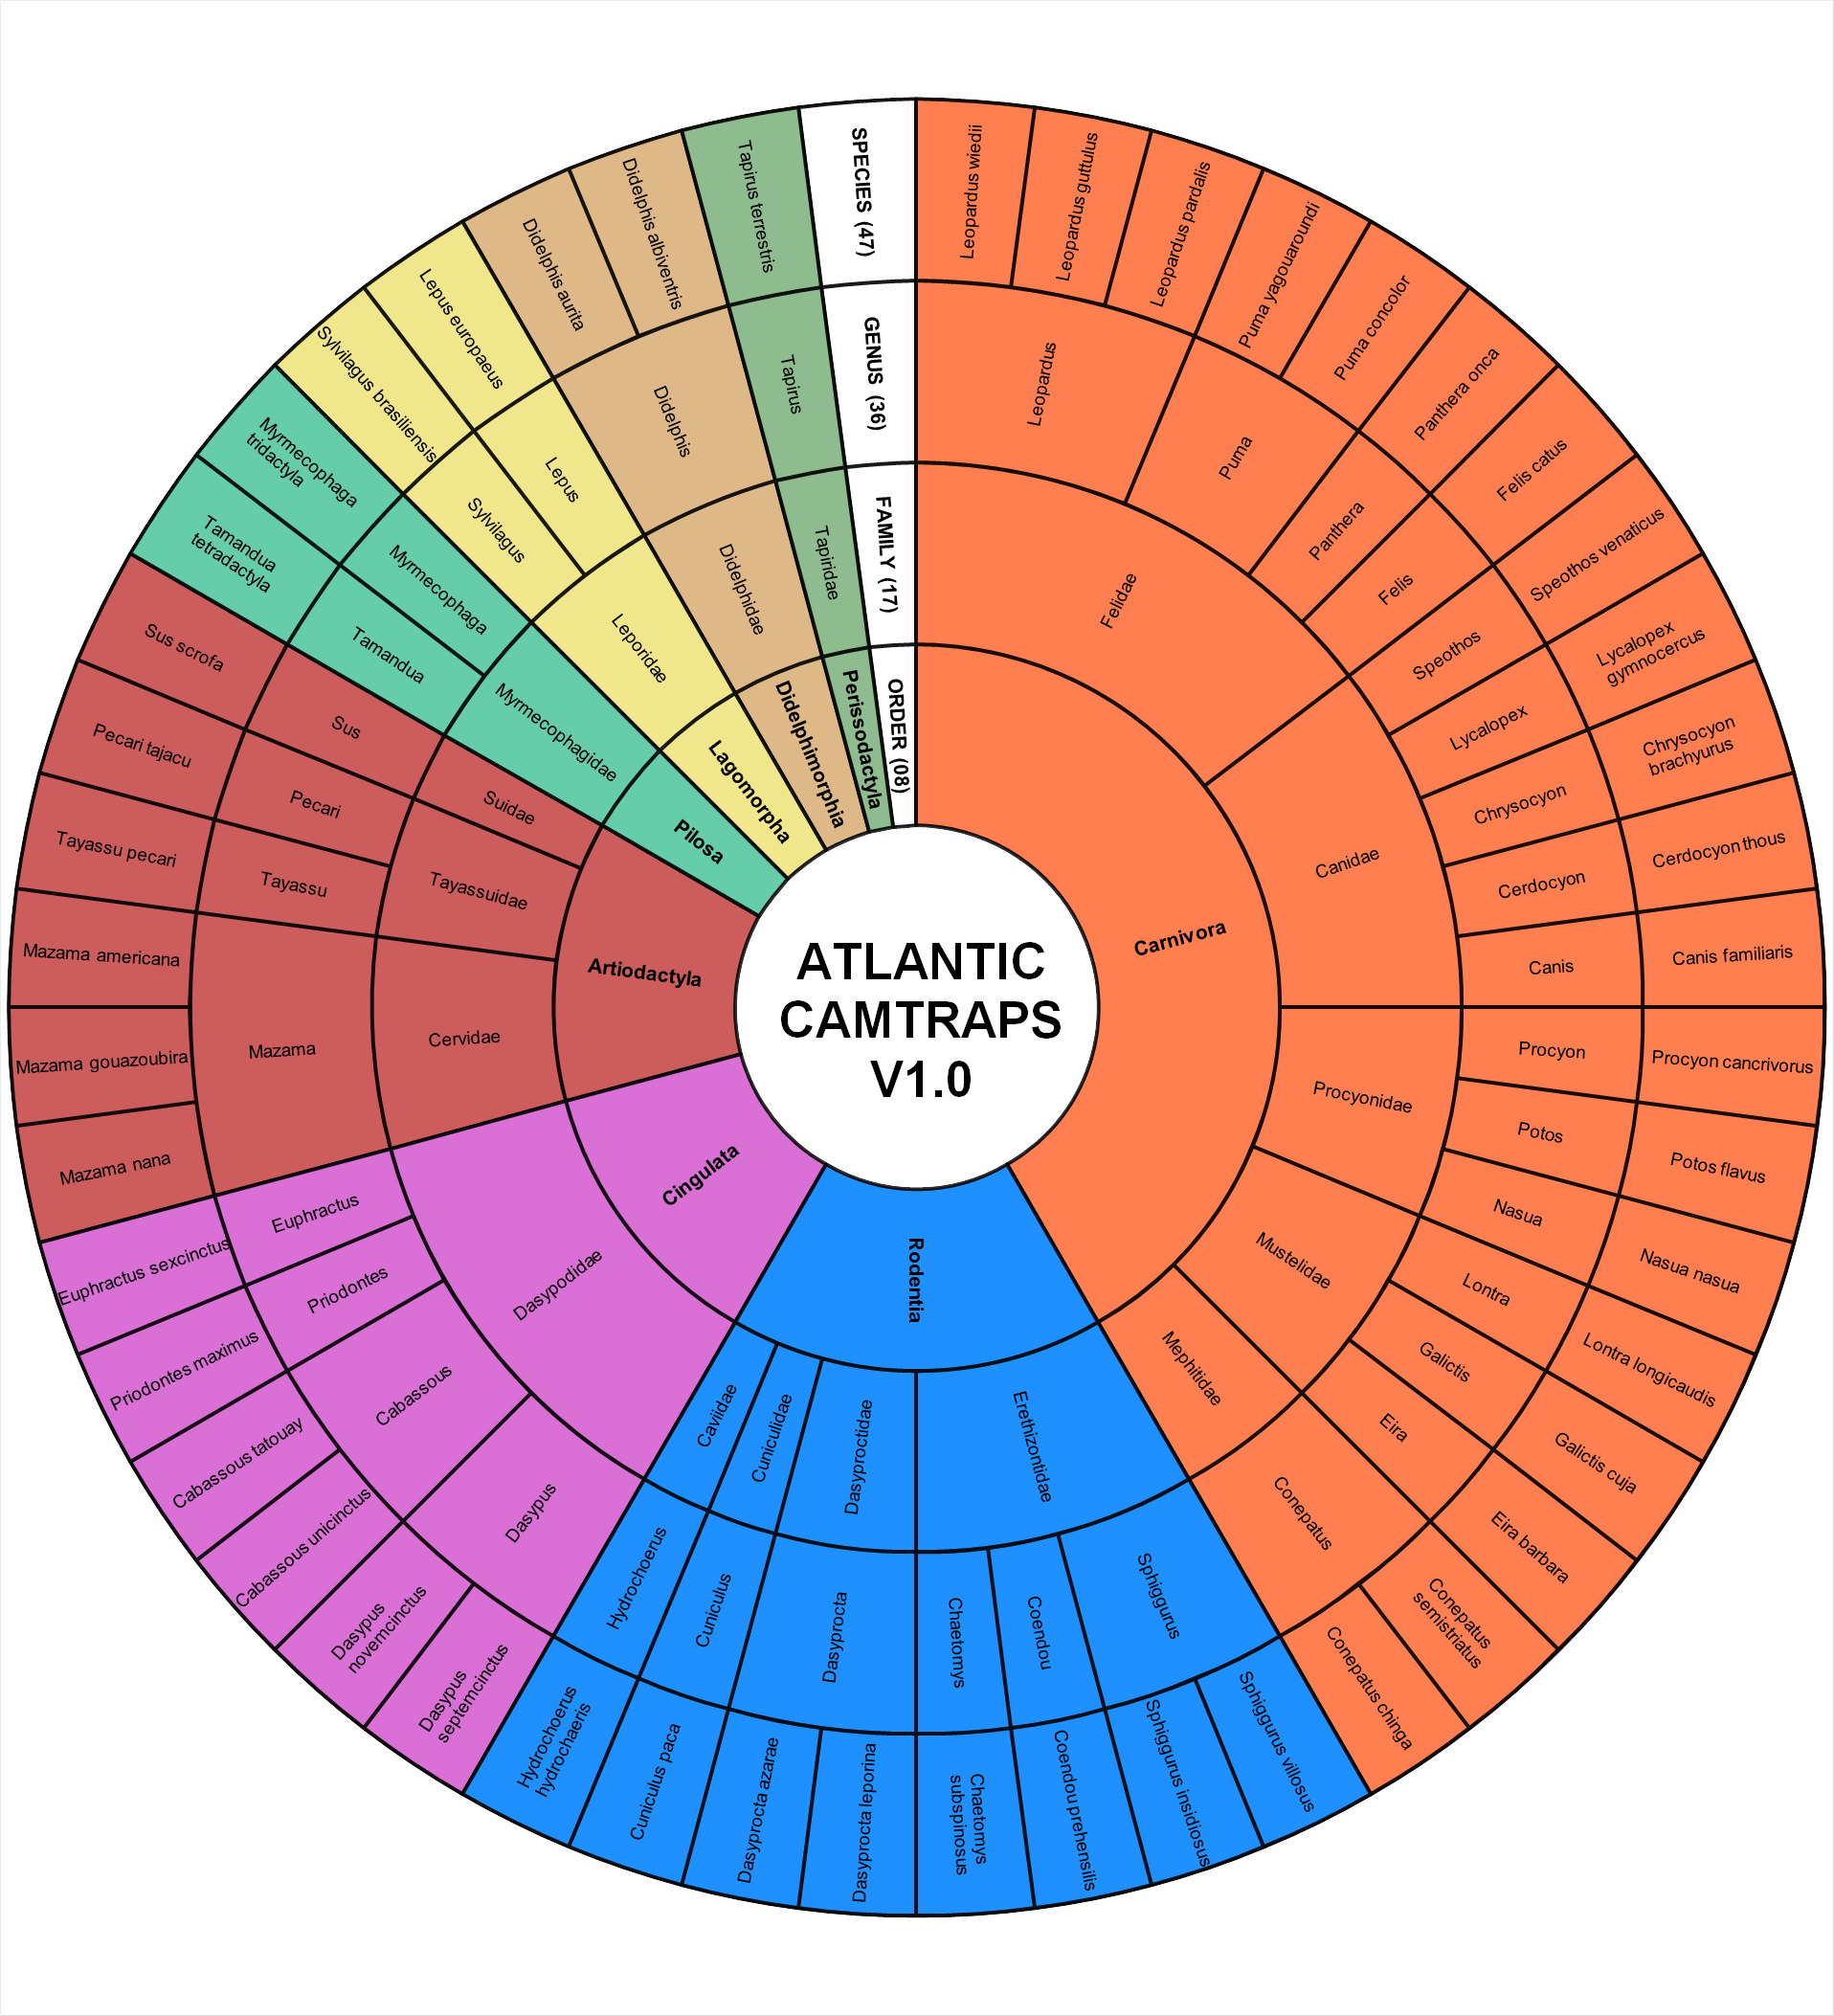
\includegraphics[width=700px]{D:/git/atlantic-series/ATLANTIC_CAMTRAP/figures/ATLANTIC_CAMTRAPS_FIG02}

\textbf{Fig. 2.} Taxonomic information levels of medium and large
terrestrial mammal species recorded in camera trap surveys within the
Atlantic Forest. Only species considered well detected by camera traps
are listed. From the 83 species reported in the database, 8 are not
listed because the identification is at genera level. Another 28 species
are not listed because they were considered opportunistic records of
species not usually detected by camera traps (primates, bats, small
rodents, and small marsupials).

\#\#\#FIGURA 03 - FREQUENCIA DE OCORRENCIA

\textbf{RM} Demanda: Casar as cores com o sunburst!\\
\textbf{pH} Eu mudei a paleta de cores. Inseri os codigos RGB para usar
igual no Excel.

\begin{Shaded}
\begin{Highlighting}[]
\FunctionTok{fct\_rev}\NormalTok{(}\FunctionTok{fct\_infreq}\NormalTok{(}\FunctionTok{factor}\NormalTok{(data}\SpecialCharTok{$}\NormalTok{species}\FloatTok{.1}\NormalTok{)))}
\end{Highlighting}
\end{Shaded}

\begin{verbatim}
##  [1] Cabassous unicinctus      Priodontes maximus       
##  [3] Conepatus chinga          Chaetomys subspinosus    
##  [5] Coendou prehensilis       Potos flavus             
##  [7] Dasypus septemcinctus     Sphiggurus insidiosus    
##  [9] Sphiggurus villosus       Speothos venaticus       
## [11] Lycalopex gymnocercus     Conepatus semistriatus   
## [13] Chrysocyon brachyurus     Dasyprocta leporina      
## [15] Lontra longicaudis        Panthera onca            
## [17] Lepus europaeus           Felis catus              
## [19] Myrmecophaga tridactyla   Tayassu pecari           
## [21] Mazama nana               Euphractus sexcinctus    
## [23] Sus scrofa                Galictis cuja            
## [25] Mazama americana          Cabassous tatouay        
## [27] Tapirus terrestris        Mazama gouazoubira       
## [29] Sylvilagus brasiliensis   Puma yagouaroundi        
## [31] Leopardus wiedii          Didelphis albiventris    
## [33] Hydrochoerus hydrochaeris Pecari tajacu            
## [35] Puma concolor             Dasyprocta azarae        
## [37] Didelphis aurita          Tamandua tetradactyla    
## [39] Leopardus pardalis        Leopardus guttulus       
## [41] Cuniculus paca            Procyon cancrivorus      
## [43] Canis familiaris          Eira barbara             
## [45] Cerdocyon thous           Nasua nasua              
## [47] Dasypus novemcinctus     
## 47 Levels: Tayassu pecari Tapirus terrestris ... Cabassous tatouay
\end{verbatim}

\begin{Shaded}
\begin{Highlighting}[]
\FunctionTok{colnames}\NormalTok{(data)[}\DecValTok{3}\NormalTok{]}\OtherTok{\textless{}{-}}\FunctionTok{paste}\NormalTok{(}\StringTok{"Order"}\NormalTok{)}
\FunctionTok{getwd}\NormalTok{()}
\end{Highlighting}
\end{Shaded}

\begin{verbatim}
## [1] "D:/git/atlantic-series/ATLANTIC_CAMTRAP/src"
\end{verbatim}

\begin{Shaded}
\begin{Highlighting}[]
\NormalTok{p}\OtherTok{\textless{}{-}} \FunctionTok{ggplot}\NormalTok{(data, }\FunctionTok{aes}\NormalTok{(}\AttributeTok{x=}\FunctionTok{reorder}\NormalTok{(species}\FloatTok{.1}\NormalTok{, }\SpecialCharTok{{-}}\NormalTok{fo) , }\AttributeTok{y=}\NormalTok{fo, }\AttributeTok{fill=}\NormalTok{Order))}\SpecialCharTok{+}
    \FunctionTok{geom\_bar}\NormalTok{(}\AttributeTok{width=}\FloatTok{0.8}\NormalTok{,}\AttributeTok{stat=}\StringTok{"identity"}\NormalTok{, }\AttributeTok{color =} \StringTok{"black"}\NormalTok{, }\AttributeTok{position=}\StringTok{"stack"}\NormalTok{, }\AttributeTok{size =}\FloatTok{0.3}\NormalTok{) }\SpecialCharTok{+} \CommentTok{\#dimgray}
    \CommentTok{\#, size = 1, shape = 1}
    \FunctionTok{theme\_bw}\NormalTok{() }\SpecialCharTok{+}
    \CommentTok{\#facet\_wrap(\textasciitilde{}order)+}
    \FunctionTok{xlab}\NormalTok{(}\StringTok{"Species"}\NormalTok{) }\SpecialCharTok{+} 
    \FunctionTok{ylab}\NormalTok{(}\StringTok{"Frequency of occurrence"}\NormalTok{)}\SpecialCharTok{+}
    \FunctionTok{theme}\NormalTok{(}\AttributeTok{legend.position=}\StringTok{"top"}\NormalTok{)}\SpecialCharTok{+}
    \FunctionTok{theme}\NormalTok{(}\AttributeTok{axis.text.x =} \FunctionTok{element\_text}\NormalTok{(}\AttributeTok{angle=}\DecValTok{45}\NormalTok{, }\CommentTok{\# pH \# mudei de 90 para 45}
    \AttributeTok{vjust=}\DecValTok{1}\NormalTok{,}
    \AttributeTok{hjust =} \DecValTok{1}\NormalTok{, }\CommentTok{\# pH \# adicionei}
    \AttributeTok{family=}\StringTok{"Times"}\NormalTok{, }\AttributeTok{face=}\StringTok{"italic"}\NormalTok{, }\AttributeTok{colour=}\StringTok{"black"}\NormalTok{, }\AttributeTok{size=}\FunctionTok{rel}\NormalTok{(}\FloatTok{0.9}\NormalTok{)))}\SpecialCharTok{+}
    \FunctionTok{geom\_text}\NormalTok{(}\FunctionTok{aes}\NormalTok{(}\AttributeTok{label=}\NormalTok{iucn\_status), }\AttributeTok{position=}\FunctionTok{position\_dodge}\NormalTok{(}\AttributeTok{width=}\FloatTok{0.7}\NormalTok{), }\AttributeTok{size=}\DecValTok{3}\NormalTok{, }\AttributeTok{colour=}\StringTok{"black"}\NormalTok{, }\AttributeTok{vjust=}\SpecialCharTok{{-}}\FloatTok{0.25}\NormalTok{)}\SpecialCharTok{+}
    \FunctionTok{theme}\NormalTok{(}\AttributeTok{plot.margin =} \FunctionTok{unit}\NormalTok{(}\FunctionTok{c}\NormalTok{(}\FloatTok{0.5}\NormalTok{,}\FloatTok{0.5}\NormalTok{,}\FloatTok{0.5}\NormalTok{,}\DecValTok{1}\NormalTok{),}\StringTok{"cm"}\NormalTok{))}

\NormalTok{cores}\OtherTok{\textless{}{-}}\FunctionTok{c}\NormalTok{(}\StringTok{"indianred1"}\NormalTok{ , }\CommentTok{\# pH \# artiodactyla mudar para indianred \#cd5c5c rgb(205,92,92)}
    \StringTok{"coral"}\NormalTok{,  }\CommentTok{\# pH \# carnivora \#ff7f50 rgb(255,127,80)}
    \StringTok{"orchid"}\NormalTok{ , }\CommentTok{\# pH \# cingulata mudar para orchid }
    \StringTok{"burlywood"}\NormalTok{, }\CommentTok{\# pH \# didelphimorphia \#deb887 rgb(222,184,135)}
    \StringTok{"khaki"}\NormalTok{, }\CommentTok{\# pH \# lagomorpha mudar para khaki \#f0e68c rgb(240,230,140)}
    \StringTok{"darkseagreen"}\NormalTok{, }\CommentTok{\# pH \#  perisodactyla mudar para darkseagreen \#8fbc8f rgb(143,188,143)}
    \StringTok{"mediumaquamarine"}\NormalTok{, }\CommentTok{\# pH \# pilosa \#66cdaa rgb(102,205,170)   }
    \StringTok{"dodgerblue"}\NormalTok{ ) }\CommentTok{\# pH \#  rodentia mudar para dodger blue \#1e90ff rgb(30,144,255)}
    \CommentTok{\#png(filename= "Fig3\_v19.png", res= 300,  height= 16, width=26, unit="cm")}
    \CommentTok{\#p+ scale\_fill\_manual(values=cores)}
    \CommentTok{\#dev.off()}

\CommentTok{\# pH \#  mesmo que acima, mas usando os codigos}
    
\NormalTok{    cores}\OtherTok{\textless{}{-}}\FunctionTok{c}\NormalTok{(}\StringTok{"\#cd5c5c"}\NormalTok{ , }\CommentTok{\# pH \# artiodactyla mudar para indianred \#cd5c5c rgb(205,92,92)}
             \StringTok{"\#ff7f50"}\NormalTok{,  }\CommentTok{\# pH \# carnivora \#ff7f50 rgb(255,127,80)}
             \StringTok{"\#da70d6"}\NormalTok{ , }\CommentTok{\# pH \# cingulata mudar para orchid \#da70d6 rgb(218,112,214)}
             \StringTok{"\#deb887"}\NormalTok{, }\CommentTok{\# pH \# didelphimorphia \#deb887 rgb(222,184,135)}
             \StringTok{"\#f0e68c"}\NormalTok{, }\CommentTok{\# pH \# lagomorpha mudar para khaki \#f0e68c rgb(240,230,140)}
             \StringTok{"\#8fbc8f"}\NormalTok{, }\CommentTok{\# pH \#  perisodactyla mudar para darkseagreen \#8fbc8f rgb(143,188,143)}
             \StringTok{"\#66cdaa"}\NormalTok{, }\CommentTok{\# pH \# pilosa \#66cdaa rgb(102,205,170)   }
             \StringTok{"\#1e90ff"}\NormalTok{ ) }\CommentTok{\# pH \# rodentia mudar para dodger blue \#1e90ff rgb(30,144,255)}
    
    \CommentTok{\#png(filename= "Fig3\_v20.png", res= 300,  height= 16, width=26, unit="cm")}
    \CommentTok{\#p+ scale\_fill\_manual(values=cores)}
    \CommentTok{\#dev.off()}
\end{Highlighting}
\end{Shaded}

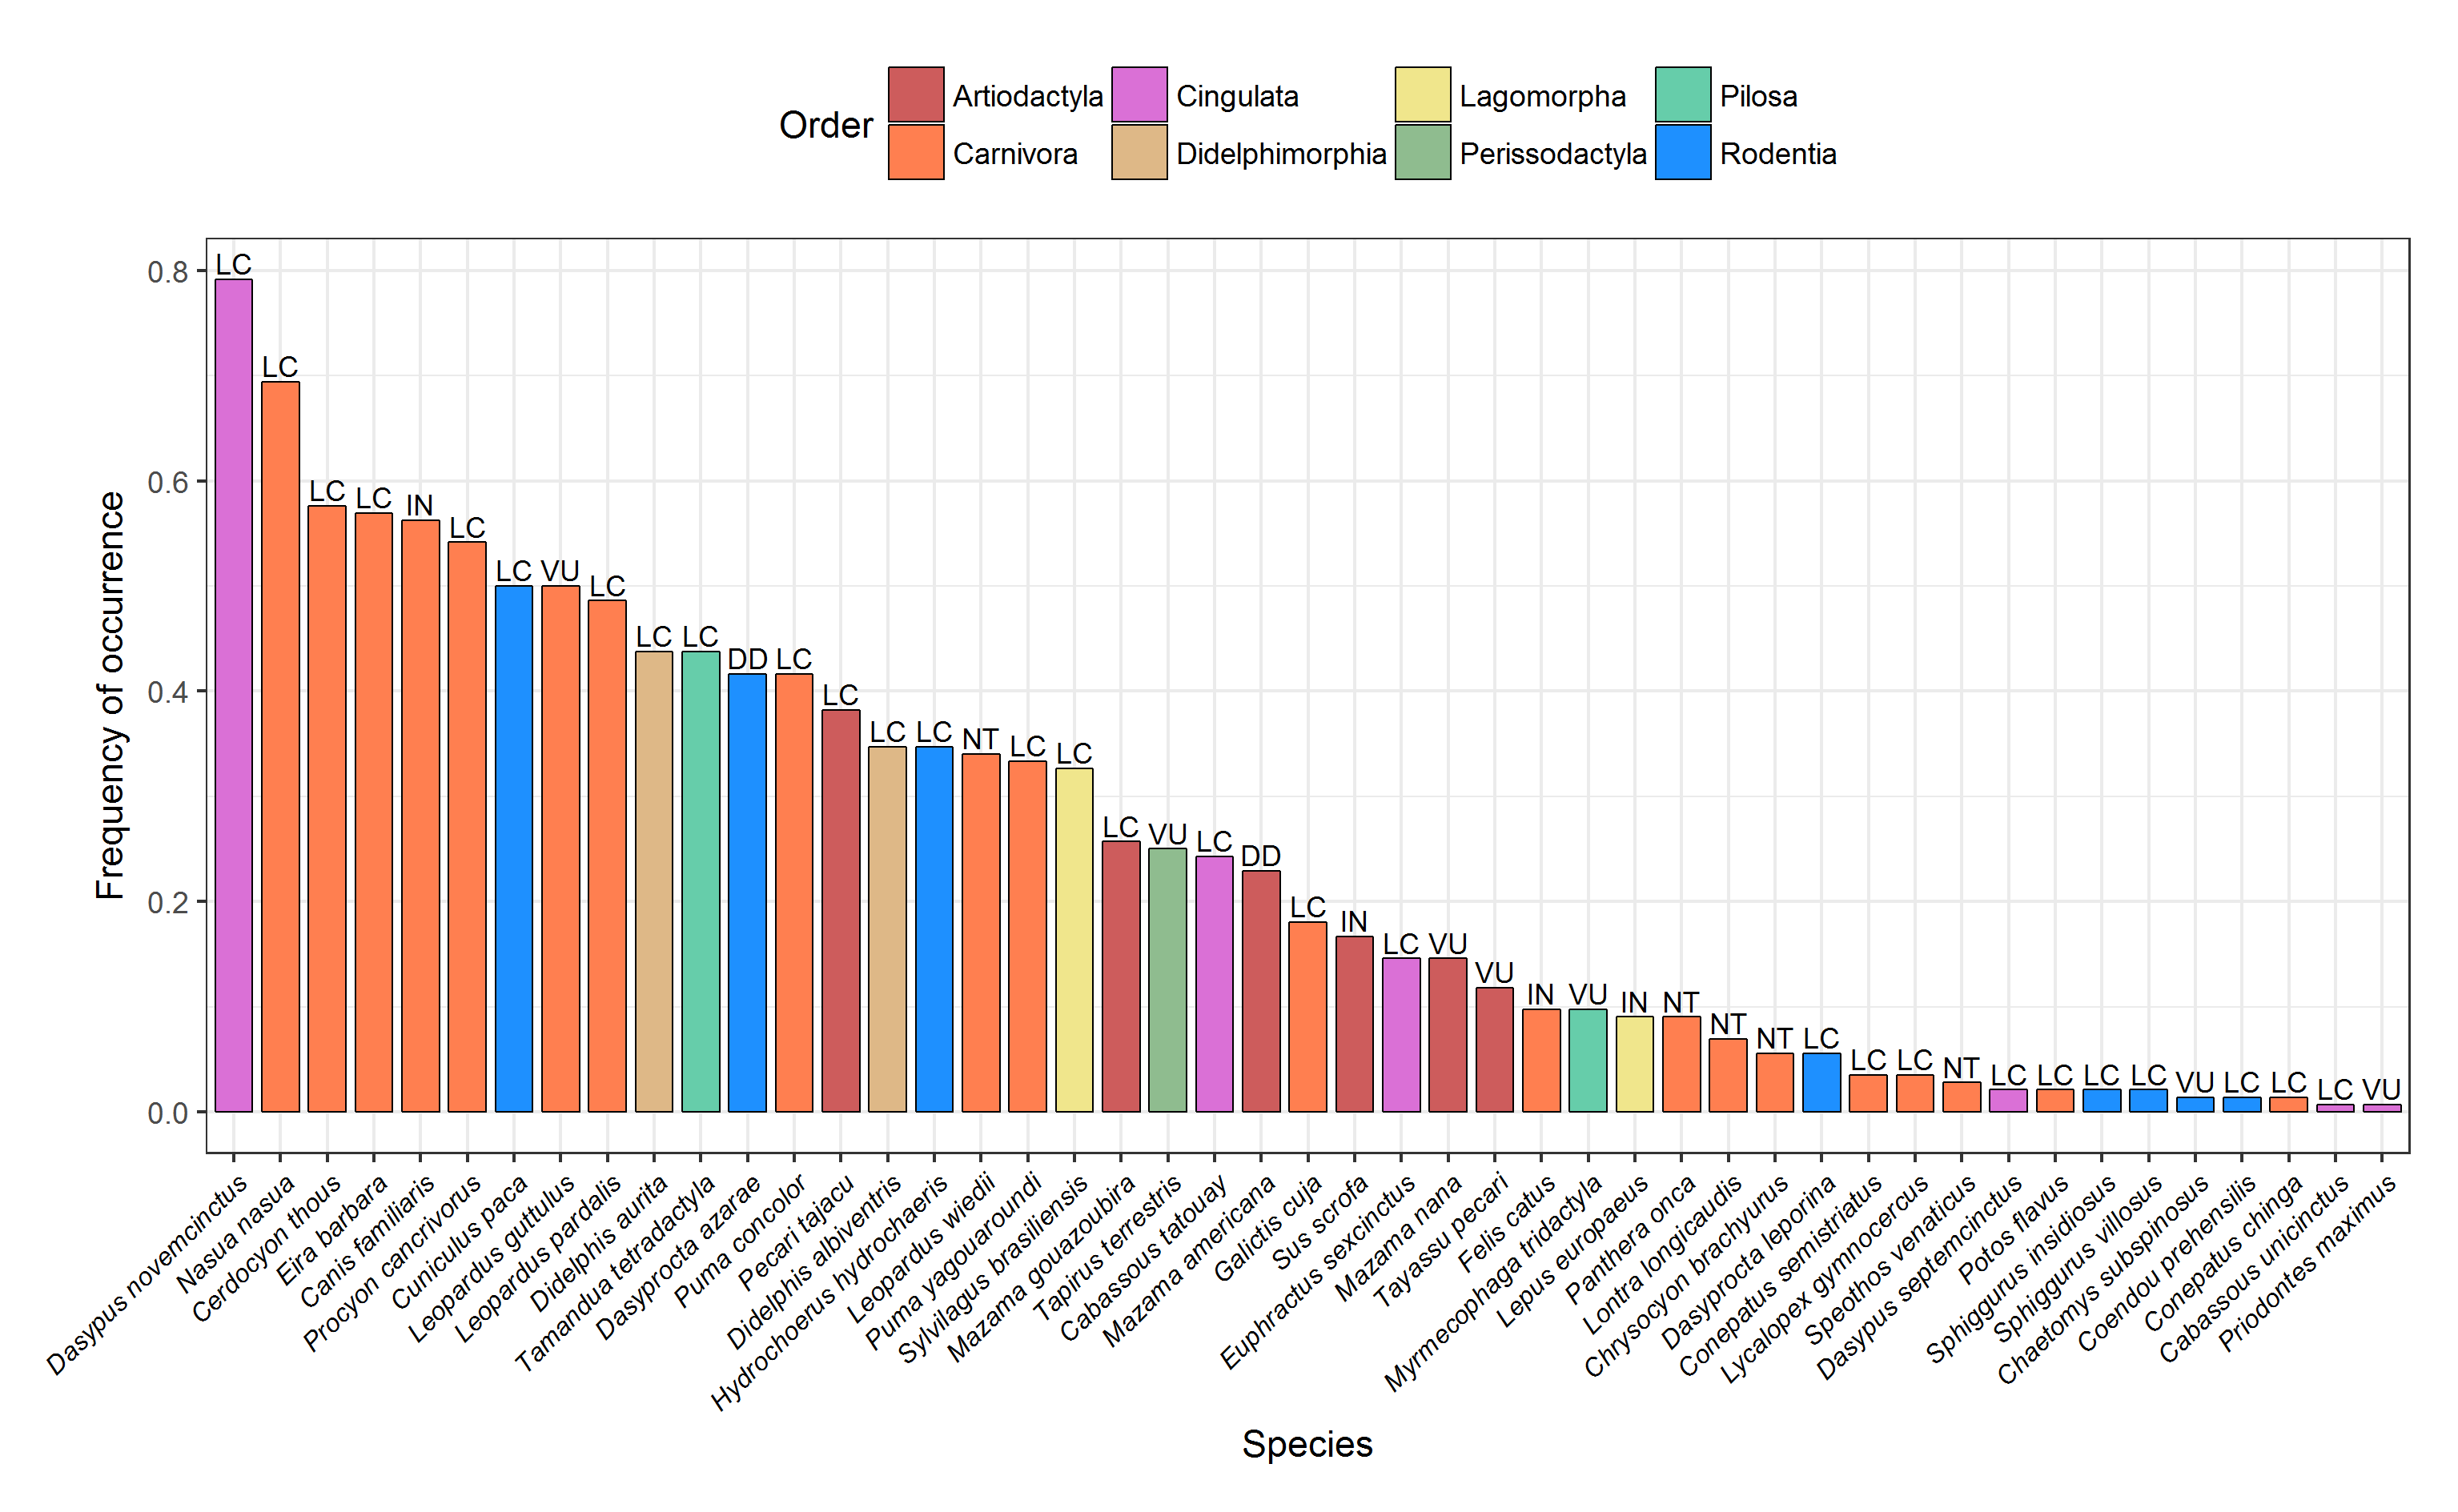
\includegraphics[width=700px]{D:/git/atlantic-series/ATLANTIC_CAMTRAP/figures/ATLANTIC_CAMTRAPS_FIG03}

\textbf{Fig. 3.} Distribution of frequencies of occurrence of the main
species evaluated in ATLANTIC-CAMTRAPS, and their status in the 2017
IUCN Red list of threatened species. LC = least concern, NT = near
threatened, VU = vulnerable, EN = endangered, CR = critically
endangered, DD = data deficient, and IN = invasive species (not an IUCN
category).

\hypertarget{figura-04---mapa}{%
\subsubsection{FIGURA 04 - MAPA}\label{figura-04---mapa}}

O mapa foi feito no ArcMap

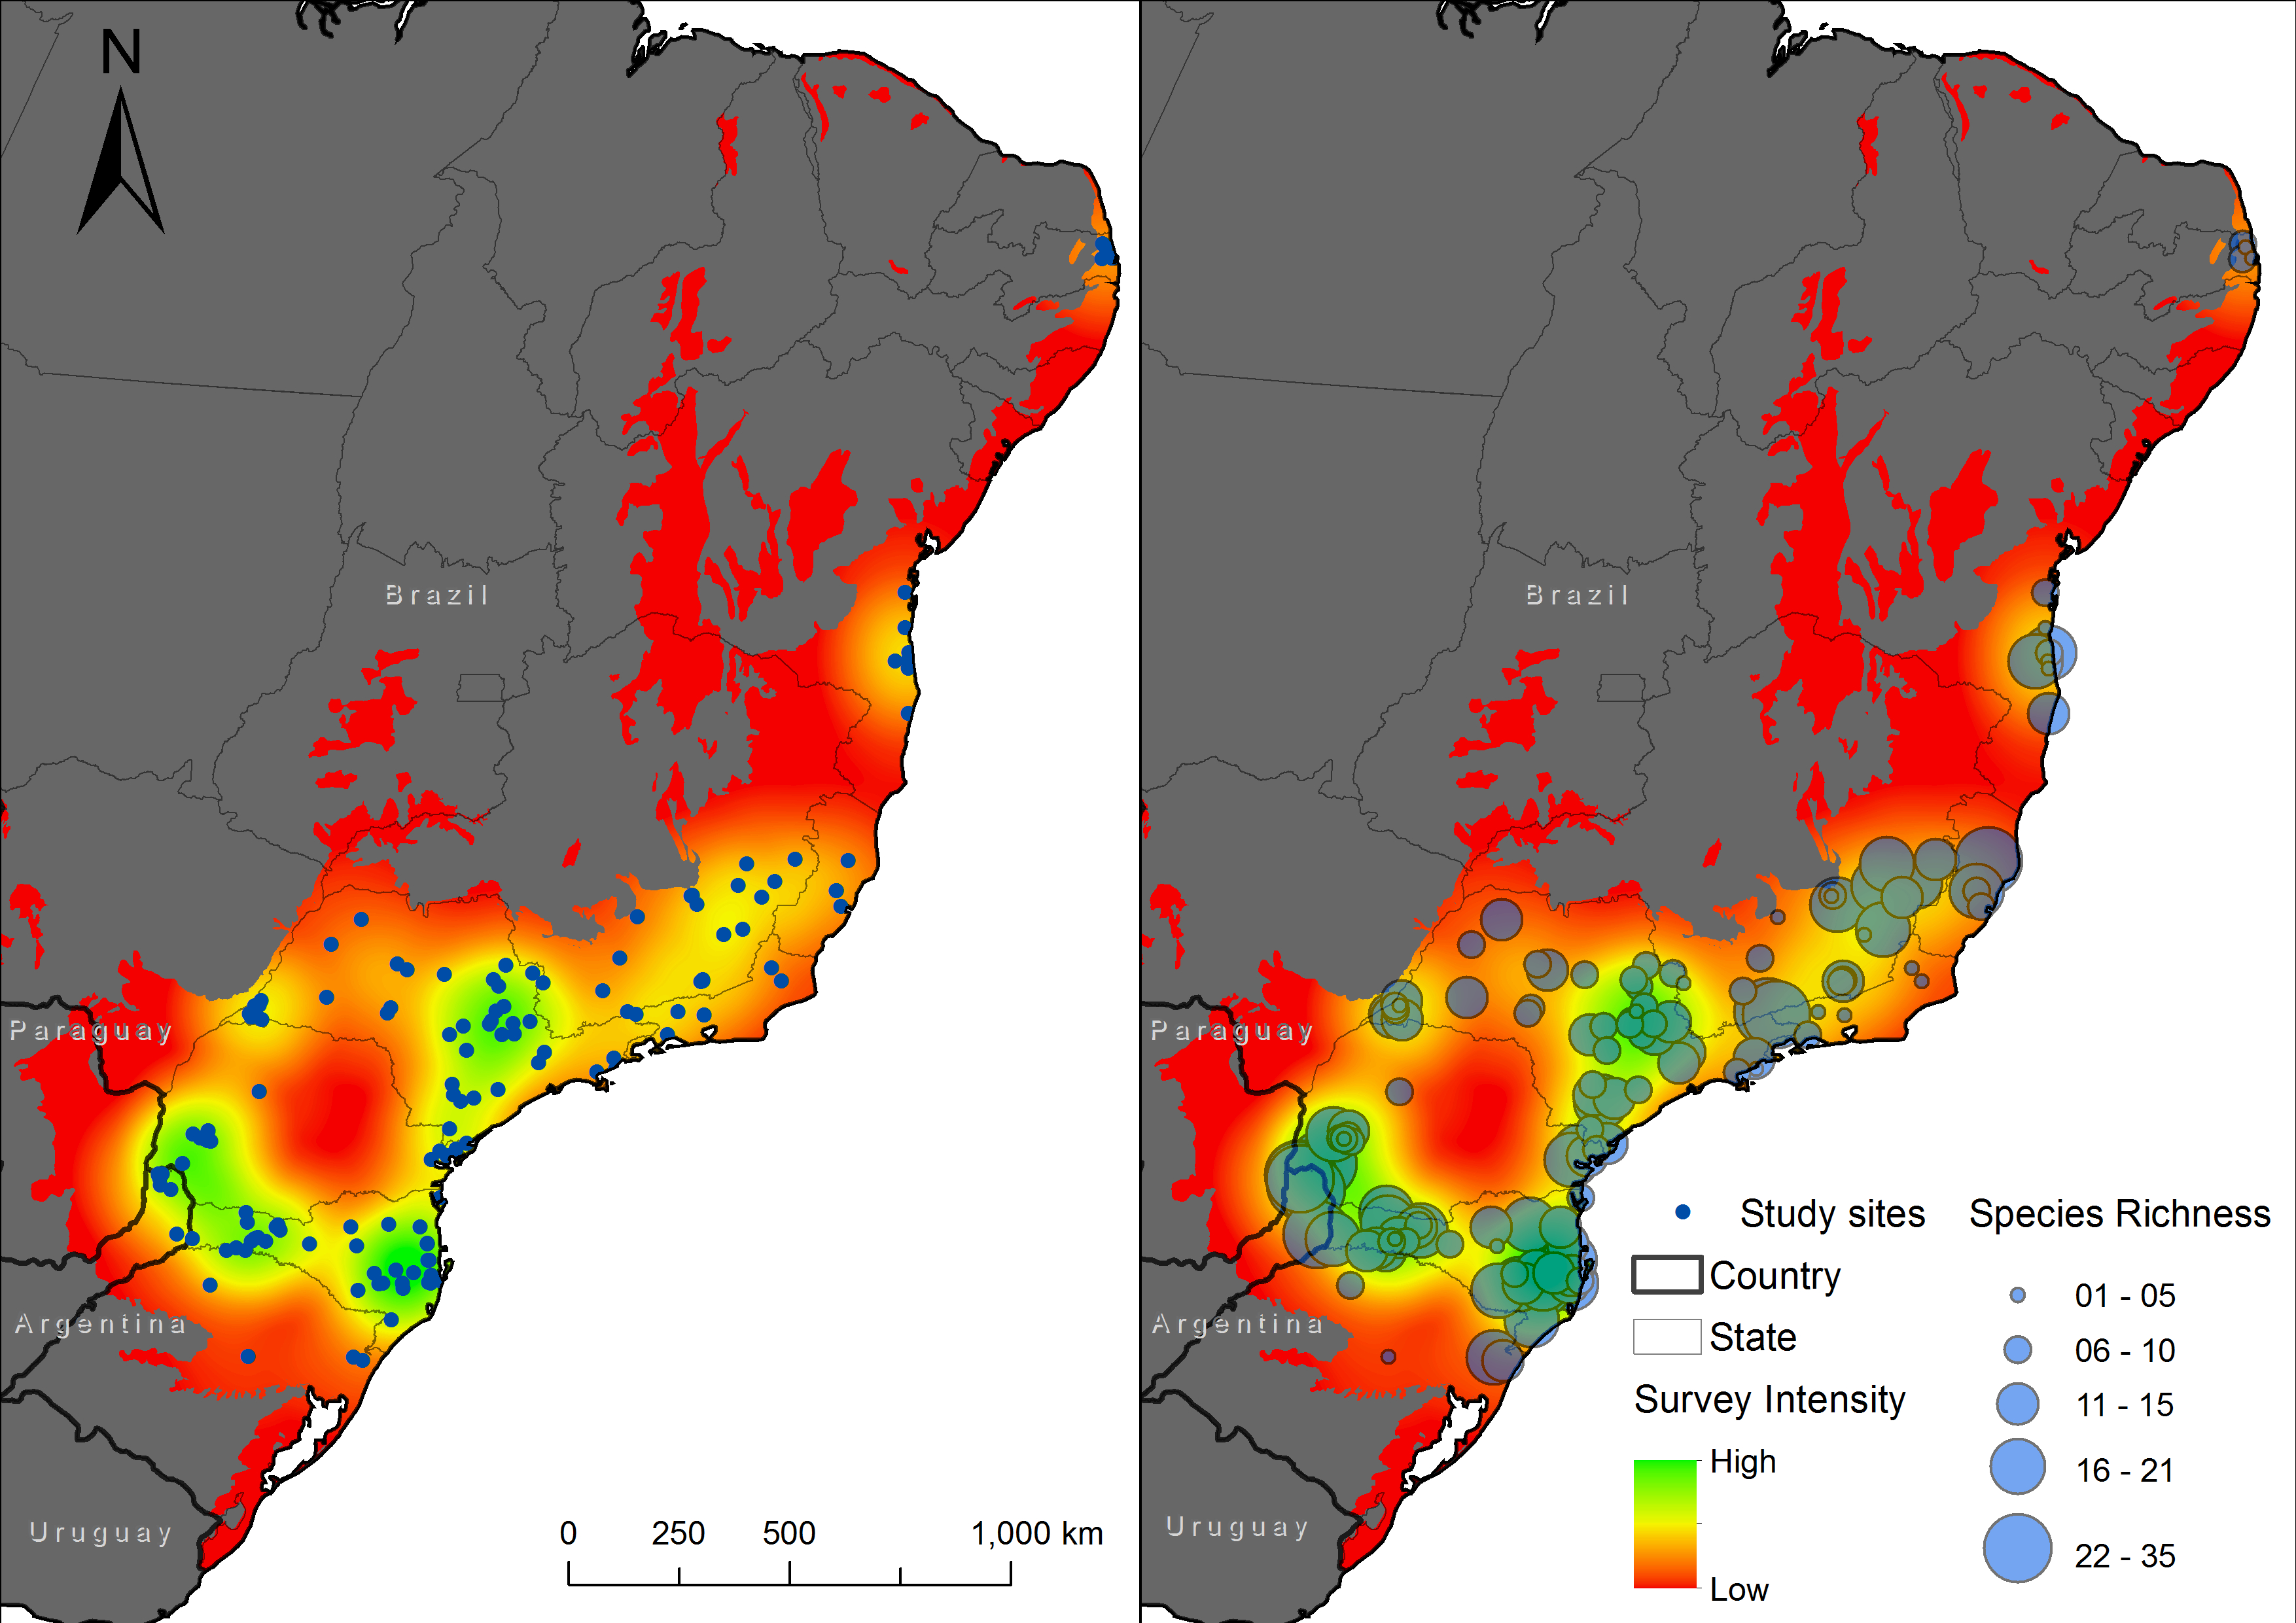
\includegraphics[width=700px]{D:/git/atlantic-series/ATLANTIC_CAMTRAP/figures/ATLANTIC_CAMTRAPS_FIG04}

\textbf{Fig. 4.} Distribution of taxonomic richness and sampling effort
across Atlantic Forest sites where camera traps were used for sampling
of medium and large terrestrial mammal species. Opportunistic records
(see the text) were removed from this analysis.

\end{document}
